\documentclass[a4paper,11pt]{amsart}
\usepackage{amssymb}
\usepackage{graphicx}
\usepackage{tkz-graph}

\parskip 1ex
\parindent 0 pt

\newcounter{temp}
\newcounter{prob_counter}
\newcounter{sprob_counter}

\newenvironment{problem}
{\begin{list}{{\bf \arabic{prob_counter}}}{
      \usecounter{prob_counter}
      \addtolength{\labelsep}{.6ex}
      \addtolength{\itemsep}{4.3ex}
      \setlength{\leftmargin}{1.4em}}
      \setcounter{prob_counter}{\value{temp}}
}
{\setcounter{temp}{\value{prob_counter}}
  \end{list}
}

\newenvironment{subprob}
{
  \begin{list}{{\bf \alph{sprob_counter}}}{
      \usecounter{sprob_counter}
      \addtolength{\labelsep}{.6ex}
      \addtolength{\itemsep}{.5ex}
      \setlength{\leftmargin}{1.7em}}
}
{\end{list}}

\newenvironment{solution}{\textbf{Solution.}}{\qed}

\newcommand{\rubrik}[1]{\bigskip \begin{center}{\bf #1}\end{center} \medskip}

\newcommand{\NN}{\mathbb{N}}
\newcommand{\ZZ}{\mathbb{Z}}
\newcommand{\QQ}{\mathbb{Q}}
\newcommand{\RR}{\mathbb{R}}




\begin{document}

\pagestyle{empty}
\thispagestyle{empty}

{\small{\sc\noindent
        Arnaldur Bjarnason ({\tt arnaldur15@ru.is}) and Árni Dagur Guðmundsson ({\tt arnidg@protonmail.ch})
}}

\rubrik{PROBLEM SET 3 (T-445-GRTH)}

You need to collect $\bf 65$ points to get a full score {\bf but} you cannot get more than {\bf X} points (in total) from a problem section with annotation {\bf max X}.

% {\bf Please make sure to:}\\
% 1. Write your name/email(s) on your work (replace my name above).\\
% 2. Write your answers in \texttt{{\textbackslash}begin\{solution\} ... {\textbackslash}end\{solution\}} blocks given after each problem. Turn in a single \LaTeX-generated pdf.\\
% 3. Write clear and concise proofs: points may be deducted for vagueness.







\section{Connectivity and Cuts ({\bf max 32})}

Below, $\mathcal{B}(G)$ denotes the set of blocks of graph $G$.

\begin{problem}
 \item (5 points) Show that a vertex $u$ in a graph $G$ is a cut-vertex if, and only if, there are vertices $v, w \in V(G) \setminus _{\{u\}}$ such that every path between $v$ and $w$ contains the vertex $u$.
\end{problem}
\begin{solution}
  If every path between $v$ and $w$ is of the form $\{v,\dots,u,\dots,w\}$ then the removal of $u$ means that there are no paths between $v$ and $w$ and thus there are at least one more component than before the removal and $u$ is a cut-vertex. Conversely, if $u$ is a cut-vertex there must be a $v$ and $w$ in seperate components in $G \setminus _{\{u\}}$ that are in the same component in $G$ and as there are no paths in the first case and at least one in the latter, all paths between $v$ and $w$ must contain $u$.
\end{solution}


\begin{problem}
 \item (5 points) Show that if $G$ is a graph on $n$ vertices and $m$ edges, we have:
 \[
   \kappa'(G) \le \left\lfloor \frac{2m}{n} \right\rfloor .
 \]
\end{problem}
\begin{solution}
  Recall the handshaking theorem, which states that:
  \[
    \sum_{v \in V(G)}{d(v)} = 2m
  \]
  We thus have:
  \[
      \frac{2m}{n} =  \frac{\sum_{v \in V(G)}{d(v)}}{|V(G)|} = \overline{d}(G) = \text{average degree in G}
  \]
  Finally, since
  \begin{align*}
    \kappa'(G) &\leq \delta(G)     & \text{and} &&    \delta(G) \leq \lfloor\overline{d}(G)\rfloor
  \end{align*}
  we have:
  \[
    \kappa'(G) \leq \lfloor\overline{d}(G)\rfloor = \left\lfloor \frac{2m}{n} \right\rfloor
  \]

\end{solution}


\begin{problem}
 \item (5 points) Show that for all $1 \le k \le k'$ there is a graph with $\kappa(G) = k$ and $\kappa'(G) = k'$.
\end{problem}
\begin{solution}
  Let $K_n \subset G$ where $n > k'$. Let there be a vertex $u$ such that $G \setminus _{\{u\}} = K_n$. When $u$ is connected to $i$ vertices by a single edge and one vertex by $j$ edges, where $i \in \NN \cup \{0\}, j \in \NN$. Then we have $k = i + 1$ and $k' = i + j$ and since $1 \le i + 1 \le i + j$, there exists a graph which satisfies the condition.
\end{solution}

\begin{problem}
 \item (5 points) Consider a simple $r$-regular graph $G$ with $\kappa(G) = 1$.
 Prove that $\kappa'(G) \leq \lfloor r/2 \rfloor$.
\end{problem}
\begin{solution}
  Since $\kappa(G) = 1$, $G$ must contain a cut-vertex $v$. Let $G' = G - v$.
  Since $v$ is a cut-vertex, $G'$ must contain at least two components. From
  that follows that there must exist a component in $G'$ that is connected to
  $v$ with at most $\lfloor r/2 \rfloor$ edges. Removing said edges disconnects
  $G$. Ergo: $\kappa'(G) \leq \lfloor r/2 \rfloor$.
\end{solution}

\begin{problem}
 \item (10 points) Let $G$ be a connected graph. Show that if $C \subseteq E(G)$ has an even number of edges in common with every edge cut of $G$, then $C$ is an edge-disjoint union of cycles.
\end{problem}
\begin{solution}
  Me and my peers have a hard time understanding this question but as I understand it it is false. Let $G$ be two cliques $c$ and $x$ which are isomorphic to eachother and $K_9$. There are two additional edges s.t. the edge cut $X = \{\{c_1,x_1\},\{c_2,x_2\}\} \in G$. If $C = X$, $C$ is not an edge-disjoint union of cycles but $C \subseteq E(G)$ has an even number of edges in common with every edge cut of $G$.
\end{solution}





\begin{problem}
  \item (5 points) For $n \ge 2$, show that for any connected $n$-vertex graph $G$, $|\mathcal{B}(G)|\le n-1$.
 Moreover, show that such a graph has exactly $n-1$ blocks if, and only if, it is a tree on $n$ vertices.
\end{problem}
\begin{solution}
\end{solution}



\begin{problem}
\item (8 points) For a graph $G$, define its \textit{block graph} $B(G)$ as the graph with vertex set $\mathcal{B}(G)$, where two blocks $B_1$ and $B_2$ are adjacent if, and only if, $B_1 \cap B_2 \ne \varnothing$.
 Show that in the graph $B(G)$, each block is a complete subgraph.
\end{problem}
\begin{solution}
  Each vertex in $B(G)$ corresponds to a block in $G$ and each edge corresponds to a pair of blocks that are connected through a cut-vertex. As all blocks that contain a cut-vertex $v$ must share that vertex with each other block containing $v$, they must all have an edge connecting them in $B(G)$. This means that each cut-vertex $v$ in $G$ must correspond to a $E(K_n)$ subgraph where $n$ is the number of components of $G \setminus _{\{v\}}$.
\end{solution}



\begin{problem}
\item (10 points) Let $G$ be a connected graph. For each vertex $u \in V(G)$, let $b(u)$ denote the number of blocks in $G$ that contain $u$. Show that the number of blocks of $G$ is given by
 $
  |\mathcal{B}(G)| = 1 + \sum_{u \in V(G)} (b(u) - 1).
 $
\end{problem}
\begin{solution}
  Let our inductive hypothesis be that:
  \[
    |\mathcal{B}(G)| = 1 + \sum_{u \in V(G)} (b(u) - 1)
  \]

  Basis step: (trivial)
  \[
    |\mathcal{B}(G)| = 1 = 1 + \sum_{u \in V(G)} (b(u) - 1)
  \]

  Recursive step: Let's add a block to $G$ to create $N$. Since our graph must
  be connected, there must exist one and only one $v \in V(G),\ b_{G}(v) =
  b_{N}(v) - 1$. Thus we have that:
  \[
    \sum_{u \in V(N)} (b(u) - 1) = 1 + \sum_{u \in V(G)} (b(u) - 1)
  \]
  Ergo:
  \[
    |\mathcal{B}(N)| = 2 + \sum_{u \in V(G)} (b(u) - 1) = |\mathcal{B}(G)| + 1
  \]

  Which proves our inductive hypothesis.
  % Let's observe that $\sum_{v \in V(c)}{b(v)-1}$ is the number of blocks
  % adjacent to block $c$. We can start at any block $s \in \mathcal{B(G)}$ and
  % recursively
\end{solution}



\begin{problem}
\item (6 points) Prove that for a simple 2-connected graph $G$ and an edge $e\in E(G)$, either $G-e$ or $G/e$ is 2-connected.
\end{problem}
\begin{solution}
\end{solution}



\section{Flows ({\bf max 28})}


\begin{problem}
  \item (5 points) Give an example of a network with more than one maximum flow. Is it possible to have precisely two maximum
 flows? In general, is it possible to have finitely many maximum flows if the maximum flow is not unique?
\end{problem}
\begin{solution}
\end{solution}


\begin{problem}
 \item (10 points) Use the Ford-Fulkerson algorithm to find a maximum flow in the following network:
 \begin{center}
\includegraphics[height=4.5cm]{ff.pdf}
 \end{center}
 Prove that the flow is indeed maximum by finding a source vertex cut $S$ such that $\text{val}(f) = c^+(S)$.
\end{problem}
\begin{solution}


\[
  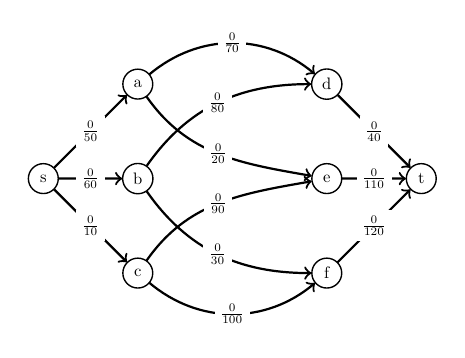
\begin{tikzpicture}[scale=0.6, every node/.style={scale=0.6},x=2cm, y=2cm]
    \GraphInit[vstyle=normal]
    \SetUpEdge[style={->}]
    \Vertex[x=0,y=1]{s}
    \Vertex[x=1,y=2]{a}
    \Vertex[x=1,y=1]{b}
    \Vertex[x=1,y=0]{c}
    \Vertex[x=3,y=2]{d}
    \Vertex[x=3,y=1]{e}
    \Vertex[x=3,y=0]{f}
    \Vertex[x=4,y=1]{t}

    \Edge[label=$\frac{0}{50 }$](s)(a)
    \Edge[label=$\frac{0}{60 }$](s)(b)
    \Edge[label=$\frac{0}{10 }$](s)(c)
    \Edge[label=$\frac{0}{70 }$,style={->,out= 40,in=140}](a)(d)
    \Edge[label=$\frac{0}{20 }$,style={->,out=-55,in=170}](a)(e)
    \Edge[label=$\frac{0}{80 }$,style={->,out= 55,in=180}](b)(d)
    \Edge[label=$\frac{0}{30 }$,style={->,out=-55,in=180}](b)(f)
    \Edge[label=$\frac{0}{90 }$,style={->,out= 55,in=190}](c)(e)
    \Edge[label=$\frac{0}{100}$,style={->,out=-40,in=220}](c)(f)
    \Edge[label=$\frac{0}{40 }$](d)(t)
    \Edge[label=$\frac{0}{110}$](e)(t)
    \Edge[label=$\frac{0}{120}$](f)(t)
  \end{tikzpicture}\ \
  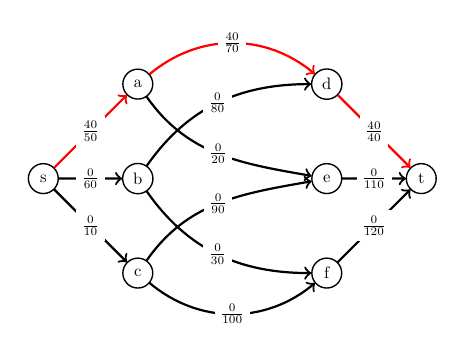
\begin{tikzpicture}[scale=0.6, every node/.style={scale=0.6},x=2cm, y=2cm]
    \GraphInit[vstyle=normal]
    \SetUpEdge[style={->}]
    \Vertex[x=0,y=1]{s}
    \Vertex[x=1,y=2]{a}
    \Vertex[x=1,y=1]{b}
    \Vertex[x=1,y=0]{c}
    \Vertex[x=3,y=2]{d}
    \Vertex[x=3,y=1]{e}
    \Vertex[x=3,y=0]{f}
    \Vertex[x=4,y=1]{t}

    \Edge[label=$\frac{40}{50 }$,color=red](s)(a)
    \Edge[label=$\frac{0}{60 }$](s)(b)
    \Edge[label=$\frac{0}{10 }$](s)(c)
    \Edge[label=$\frac{40}{70 }$,color=red,style={->,out= 40,in=140}](a)(d)
    \Edge[label=$\frac{0}{20 }$,style={->,out=-55,in=170}](a)(e)
    \Edge[label=$\frac{0}{80 }$,style={->,out= 55,in=180}](b)(d)
    \Edge[label=$\frac{0}{30 }$,style={->,out=-55,in=180}](b)(f)
    \Edge[label=$\frac{0}{90 }$,style={->,out= 55,in=190}](c)(e)
    \Edge[label=$\frac{0}{100}$,style={->,out=-40,in=220}](c)(f)
    \Edge[label=$\frac{40}{40 }$,color=red](d)(t)
    \Edge[label=$\frac{0}{110}$](e)(t)
    \Edge[label=$\frac{0}{120}$](f)(t)
  \end{tikzpicture}
\]
\[
  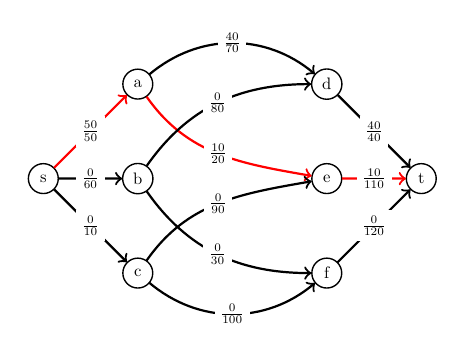
\begin{tikzpicture}[scale=0.6, every node/.style={scale=0.6},x=2cm, y=2cm]
    \GraphInit[vstyle=normal]
    \SetUpEdge[style={->}]
    \Vertex[x=0,y=1]{s}
    \Vertex[x=1,y=2]{a}
    \Vertex[x=1,y=1]{b}
    \Vertex[x=1,y=0]{c}
    \Vertex[x=3,y=2]{d}
    \Vertex[x=3,y=1]{e}
    \Vertex[x=3,y=0]{f}
    \Vertex[x=4,y=1]{t}

    \Edge[label=$\frac{50}{50 }$,color=red](s)(a)
    \Edge[label=$\frac{ 0}{60 }$](s)(b)
    \Edge[label=$\frac{ 0}{10 }$](s)(c)
    \Edge[label=$\frac{40}{70 }$,style={->,out= 40,in=140}](a)(d)
    \Edge[label=$\frac{10}{20 }$,color=red,style={->,out=-55,in=170}](a)(e)
    \Edge[label=$\frac{ 0}{80 }$,style={->,out= 55,in=180}](b)(d)
    \Edge[label=$\frac{ 0}{30 }$,style={->,out=-55,in=180}](b)(f)
    \Edge[label=$\frac{ 0}{90 }$,style={->,out= 55,in=190}](c)(e)
    \Edge[label=$\frac{ 0}{100}$,style={->,out=-40,in=220}](c)(f)
    \Edge[label=$\frac{40}{40 }$](d)(t)
    \Edge[label=$\frac{10}{110}$,color=red](e)(t)
    \Edge[label=$\frac{ 0}{120}$](f)(t)
  \end{tikzpicture}\ \
  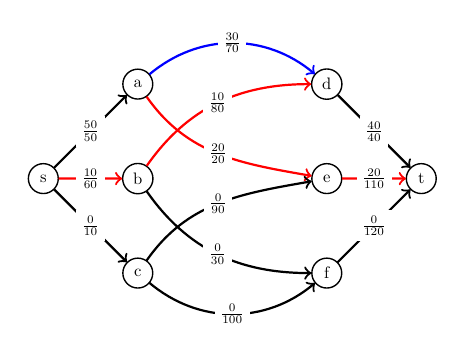
\begin{tikzpicture}[scale=0.6, every node/.style={scale=0.6},x=2cm, y=2cm]
    \GraphInit[vstyle=normal]
    \SetUpEdge[style={->}]
    \Vertex[x=0,y=1]{s}
    \Vertex[x=1,y=2]{a}
    \Vertex[x=1,y=1]{b}
    \Vertex[x=1,y=0]{c}
    \Vertex[x=3,y=2]{d}
    \Vertex[x=3,y=1]{e}
    \Vertex[x=3,y=0]{f}
    \Vertex[x=4,y=1]{t}

    \Edge[label=$\frac{50}{50 }$](s)(a)
    \Edge[label=$\frac{10}{60 }$,color=red](s)(b)
    \Edge[label=$\frac{ 0}{10 }$](s)(c)
    \Edge[label=$\frac{30}{70 }$,color=blue,style={->,out= 40,in=140}](a)(d)
    \Edge[label=$\frac{20}{20 }$,color=red,style={->,out=-55,in=170}](a)(e)
    \Edge[label=$\frac{10}{80 }$,color=red,style={->,out= 55,in=180}](b)(d)
    \Edge[label=$\frac{ 0}{30 }$,style={->,out=-55,in=180}](b)(f)
    \Edge[label=$\frac{ 0}{90 }$,style={->,out= 55,in=190}](c)(e)
    \Edge[label=$\frac{ 0}{100}$,style={->,out=-40,in=220}](c)(f)
    \Edge[label=$\frac{40}{40 }$](d)(t)
    \Edge[label=$\frac{20}{110}$,color=red](e)(t)
    \Edge[label=$\frac{ 0}{120}$](f)(t)
  \end{tikzpicture}
\]
\[
  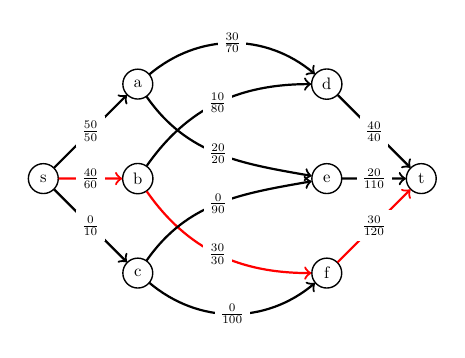
\begin{tikzpicture}[scale=0.6, every node/.style={scale=0.6},x=2cm, y=2cm]
    \GraphInit[vstyle=normal]
    \SetUpEdge[style={->}]
    \Vertex[x=0,y=1]{s}
    \Vertex[x=1,y=2]{a}
    \Vertex[x=1,y=1]{b}
    \Vertex[x=1,y=0]{c}
    \Vertex[x=3,y=2]{d}
    \Vertex[x=3,y=1]{e}
    \Vertex[x=3,y=0]{f}
    \Vertex[x=4,y=1]{t}

    \Edge[label=$\frac{50}{50 }$](s)(a)
    \Edge[label=$\frac{40}{60 }$,color=red](s)(b)
    \Edge[label=$\frac{ 0}{10 }$](s)(c)
    \Edge[label=$\frac{30}{70 }$,style={->,out= 40,in=140}](a)(d)
    \Edge[label=$\frac{20}{20 }$,style={->,out=-55,in=170}](a)(e)
    \Edge[label=$\frac{10}{80 }$,style={->,out= 55,in=180}](b)(d)
    \Edge[label=$\frac{30}{30 }$,color=red,style={->,out=-55,in=180}](b)(f)
    \Edge[label=$\frac{ 0}{90 }$,style={->,out= 55,in=190}](c)(e)
    \Edge[label=$\frac{ 0}{100}$,style={->,out=-40,in=220}](c)(f)
    \Edge[label=$\frac{40}{40 }$](d)(t)
    \Edge[label=$\frac{20}{110}$](e)(t)
    \Edge[label=$\frac{30}{120}$,color=red](f)(t)
  \end{tikzpicture}\ \
  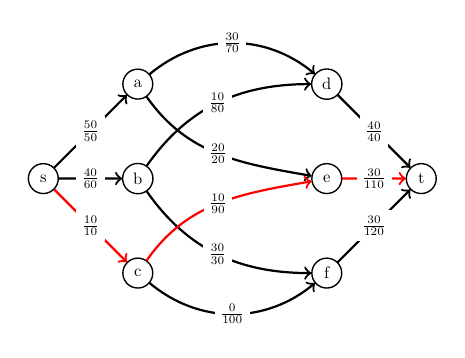
\begin{tikzpicture}[scale=0.6, every node/.style={scale=0.6},x=2cm, y=2cm]
    \GraphInit[vstyle=normal]
    \SetUpEdge[style={->}]
    \Vertex[x=0,y=1]{s}
    \Vertex[x=1,y=2]{a}
    \Vertex[x=1,y=1]{b}
    \Vertex[x=1,y=0]{c}
    \Vertex[x=3,y=2]{d}
    \Vertex[x=3,y=1]{e}
    \Vertex[x=3,y=0]{f}
    \Vertex[x=4,y=1]{t}

    \Edge[label=$\frac{50}{50 }$](s)(a)
    \Edge[label=$\frac{40}{60 }$](s)(b)
    \Edge[label=$\frac{10}{10 }$,color=red](s)(c)
    \Edge[label=$\frac{30}{70 }$,style={->,out= 40,in=140}](a)(d)
    \Edge[label=$\frac{20}{20 }$,style={->,out=-55,in=170}](a)(e)
    \Edge[label=$\frac{10}{80 }$,style={->,out= 55,in=180}](b)(d)
    \Edge[label=$\frac{30}{30 }$,style={->,out=-55,in=180}](b)(f)
    \Edge[label=$\frac{10}{90 }$,color=red,style={->,out= 55,in=190}](c)(e)
    \Edge[label=$\frac{ 0}{100}$,style={->,out=-40,in=220}](c)(f)
    \Edge[label=$\frac{40}{40 }$](d)(t)
    \Edge[label=$\frac{30}{110}$,color=red](e)(t)
    \Edge[label=$\frac{30}{120}$](f)(t)
  \end{tikzpicture}
\]
Thus we have that the maximum flow of the graph is $100$.\\
\[
  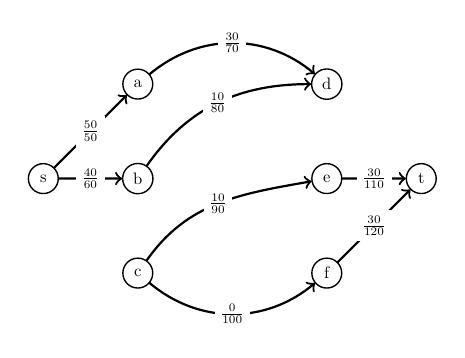
\begin{tikzpicture}[scale=0.6, every node/.style={scale=0.6},x=2cm, y=2cm]
    \GraphInit[vstyle=normal]
    \SetUpEdge[style={->}]
    \Vertex[x=0,y=1]{s}
    \Vertex[x=1,y=2]{a}
    \Vertex[x=1,y=1]{b}
    \Vertex[x=1,y=0]{c}
    \Vertex[x=3,y=2]{d}
    \Vertex[x=3,y=1]{e}
    \Vertex[x=3,y=0]{f}
    \Vertex[x=4,y=1]{t}

    \Edge[label=$\frac{50}{50 }$](s)(a)
    \Edge[label=$\frac{40}{60 }$](s)(b)
%    \Edge[label=$\frac{10}{10 }$](s)(c)
    \Edge[label=$\frac{30}{70 }$,style={->,out= 40,in=140}](a)(d)
%    \Edge[label=$\frac{20}{20 }$,style={->,out=-55,in=170}](a)(e)
    \Edge[label=$\frac{10}{80 }$,style={->,out= 55,in=180}](b)(d)
%    \Edge[label=$\frac{30}{30 }$,style={->,out=-55,in=180}](b)(f)
    \Edge[label=$\frac{10}{90 }$,style={->,out= 55,in=190}](c)(e)
    \Edge[label=$\frac{ 0}{100}$,style={->,out=-40,in=220}](c)(f)
%    \Edge[label=$\frac{40}{40 }$](d)(t)
    \Edge[label=$\frac{30}{110}$](e)(t)
    \Edge[label=$\frac{30}{120}$](f)(t)
  \end{tikzpicture}\ \
  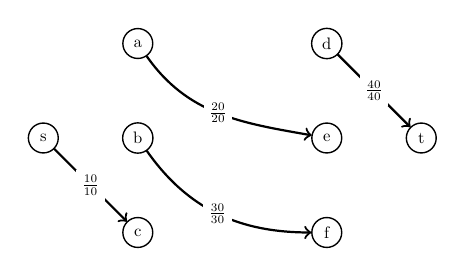
\begin{tikzpicture}[scale=0.6, every node/.style={scale=0.6},x=2cm, y=2cm]
    \GraphInit[vstyle=normal]
    \SetUpEdge[style={->}]
    \Vertex[x=0,y=1]{s}
    \Vertex[x=1,y=2]{a}
    \Vertex[x=1,y=1]{b}
    \Vertex[x=1,y=0]{c}
    \Vertex[x=3,y=2]{d}
    \Vertex[x=3,y=1]{e}
    \Vertex[x=3,y=0]{f}
    \Vertex[x=4,y=1]{t}

%    \Edge[label=$\frac{50}{50 }$](s)(a)
%    \Edge[label=$\frac{40}{60 }$](s)(b)
    \Edge[label=$\frac{10}{10 }$](s)(c)
%    \Edge[label=$\frac{30}{70 }$,style={->,out= 40,in=140}](a)(d)
    \Edge[label=$\frac{20}{20 }$,style={->,out=-55,in=170}](a)(e)
%    \Edge[label=$\frac{10}{80 }$,style={->,out= 55,in=180}](b)(d)
    \Edge[label=$\frac{30}{30 }$,style={->,out=-55,in=180}](b)(f)
%    \Edge[label=$\frac{10}{90 }$,style={->,out= 55,in=190}](c)(e)
%    \Edge[label=$\frac{ 0}{100}$,style={->,out=-40,in=220}](c)(f)
    \Edge[label=$\frac{40}{40 }$](d)(t)
%    \Edge[label=$\frac{30}{110}$](e)(t)
%    \Edge[label=$\frac{30}{120}$](f)(t)
  \end{tikzpicture}
\]
On the left is the graph after the edge cut and on the right are the saturated edges $S$ that satisfy the property $c^+(S) = \text{val}(f)$.
\end{solution}


\begin{problem}
\item (10 points) Let $\vec{G}$ be an Eulerian digraph and let $u,v \in V(\vec{G})$ be adjacent by exactly $k$ parallel directed edges with tail $u$ and head $v$. Let $\vec{G'}$ be the digraph obtained from $\vec{G}$ by removing those $k$ edges.
 Show that $\vec{G'}$ has $k$ edge-disjoint directed $v,u$-paths.
\end{problem}
\begin{solution}
\end{solution}


\begin{problem}
\item (8 points) Consider a 3-vertex-connected graph $G$ and verices $u \neq v$.
By Menger's theorem, $G$ contains three vertex-disjoint (except for endpoints) $u,v$-paths.
{\em Given} two vertex disjoint $u,v$-paths $p$ and $q$, is it always possible to find a third path $r$ that is vertex-disjoint from both $p$ and $q$?
\end{problem}
\begin{solution}
\end{solution}


\section{Planar Graphs ({\bf max 25})}


\begin{problem}
\item (5 points) Consider a simple graph $G$ on six vertices $a, b, c, d, e, f$
where each pair of vertices is adjacent except for the pairs $\{a, b \}$, $\{c, d \}$, $\{e, f \}$. Is $G$ a planar graph?
\end{problem}
\begin{solution}
  Yes! See figure \ref{fig:prob14}.
  \begin{figure}[h]
    \centering
    \includegraphics[width=0.7\linewidth]{Problem14.jpg}
    \caption{As can be seen, the graph $G$ is planar.}
    \label{fig:prob14}
  \end{figure}
\end{solution}


\begin{problem}
 \item (10 points) Euler's formula states: Every connected plane graph with $n$ vertices, $m$ edges, and $f$ faces satisfies the  equation $n - m +f = 2$.
Prove this formula inductively by using contraction of a graph by an edge.
\end{problem}
\begin{solution}
  $N_1$ satisfies euler's formula $1 - 0 + 1 = 2$ as we count the infinite face surrounding the graph. Let $G$ be a connected planar graph.
  Assume that the formula works for when $|V(G)| = n$. By contracting an edge $e \in G$, the resultant $G'$ has one less edge and vertex and thus $$(n-1) - (m-1) + f = n - 1 - m + 1 + f = n - m + f$$ and the invariant holds.
  We must also consider a single vertex with $k$ loops. Each loop adds an edge and a face and thus $1 - k + (1 + k) = 1 - k + k + 1 = 2$. The reason this is considered is that any face disjoint cycle of $G$ leaves a single loop when no edges of the cycle can be contracted anymore.
\end{solution}



\begin{problem}
\item  Prove that:
 \begin{subprob}
    \item (5 points) Every simple planar graph with no $3$-cycles has a vertex of degree at most $3$.
    \item (5 points) Every simple planar graph on $n \ge 4$ vertices has at least four vertices of degree at most $5$.
  \end{subprob}
\end{problem}
\begin{solution}
  We know that if a simple planar graph $G$ contains no triangles
  (3-cycles), we have:
  \[
    m \leq 2n - 4
  \]
  Where $m$ is the number of edges, and $n$ is the number of verteces in $G$.
  Let's assume by contradiction that $G$ contains no vertex of degree $\leq 3$.
  We have:
  \[
   4n \leq \sum_{v \in V(G)}{d(v)} = 2m \leq 4n - 8
  \]
  From that follows that $0 \leq -8$, which is a contradiction.
\end{solution}

\begin{solution}
  Let $G$ be a simple maximal planar graph. We know that $3 \leq \delta(G)$
  since $G$ is maximally planar.
  We also know that:
  \[
    m \leq 3n - 6
  \]
  Where $m$ is the number of edges, and $n$ is the number of verteces in $G$.
  Let's assume by contradiction that $G$ only contains $3$ or less verteces
  with degree $\leq 5$, we have:
  \[
    6n - 9 \leq 3*3 + (n-3)*6 \leq \sum_{v \in V(G)}{d(v)} = 2m \leq 6n - 12
  \]
  Which is a contradiction since $-9 \nleq -12$. Proving this for a maximally
  planar graph, as we just did, is sufficient; removing edges from a
  maximally planar graph $G$ can only decrease the degrees of the verteces
  of $G$.
\end{solution}


\begin{problem}
\item (5 points) Show that a simple and connected $4$-regular planar graph, where each face is bounded by exactly $3$ edges,
 must have $6$ vertices, $12$ edges and $8$ faces.
\end{problem}
\begin{solution}
\end{solution}




\end{document}

%%% Local Variables:
%%% mode: latex
%%% TeX-master: t
%%% End:
